\chapter{集合与简易逻辑}

 \section{集合}
\subsection{集合的概念}
我们在第一册中曾用到过集合的概念,如自然数所构成
的集合$\{1,2,3,\ldots\}$, 方程$x^2=4$的解所构成的集合$\{-2,2\}$
等等。那么,什么是集合呢?集合是数学中一个很根本的也
是很原始的概念,通常我们把一些确定的、彼此不同的“事
物”作为一个整体来考虑时,这个整体便说是一个\textbf{集合}。这
些事物叫做该集合的\textbf{元素}。例如:
某中学初二(一)班全体学生;小于100的全体质数;
一个生产队的全体社员;一个工厂的全部机器等等,都可分别构成一个集合。可见集合的概念是很简单
的。

对于集合这个概念,我们要注意以下几点:

第一,一个集合完全被它所含的元素所确定。至于集合
的元素之间是否具有某种相互关系,怎样排列,以及这些元
素所构成的集合是具有某种功效,单从集合的观点来看,
是一样的。例如,“一堆还没有组装的手表另件”和用“这
些另件组装好了的手表”是同一个集合。因为两者包含同样
的元素。因此,集合这个概念的要素是:\textbf{一个集合完全被它
所含的元素所确定}。

第二,集合是指构成集合的全体元素,而不是个别元
素。作为整体的集合和集合中的每个元素都是不同的。

例如,集合$A=\{a,b,c,d\}$, $A$代表的是字母$a$、$b$、
$c$、$d$的全体,而不是代表其中的个别字母,因此,作为字母
$a$、$b$、
$c$、$d$的整体的集合$A$与$A$中的个别元素如$a,b,c,d$不
能混为一谈。

第三,集合中所含的元素必须是“确定”的,是可以判
断的。例如,由“比较小的实数”的全体就不能构成一个集
合,因为到底什么叫做比较小的实数,没有判断的标准。但
是“比80小的实数”是完全可以确定的,这就有了检验一个
实数是否是这个集合的元素的标准。

任一几何图形,我们可以看作由点构成的,也就是可看
作点的集合。例如:

\textbf{圆}是同一平面上与一定点的距离等于定长的所有点的集
合(图2.1(1))。

\textbf{圆面}是同一平面上与一定点距离小于或等于定长的所有
点的集合。(图2.1(2))。

\begin{figure}[htp]
	\centering
	\begin{tikzpicture}[scale=.7]
		\begin{scope}
			\draw (0,0) circle (2);
\draw[ultra thick] (0,0)node[below]{$O$}--node[left]{$r$}(45:2);		
\node at (0,-3){(1)圆};	
		\end{scope}
		\begin{scope}[xshift=6cm]
			\draw[pattern=north west lines] (0,0) circle (2);
\draw[ultra thick] (0,0)node[below, fill=white]{$O$}--(45:2);	
			\node at (60:1.5) [left, rotate=45, fill=white]{$r$};
			
			\node at (0,-3){(2)圆面};
		\end{scope}
	\end{tikzpicture}	
	\caption{}
\end{figure}

我们通常用大写字母$A,B,C,\ldots$等表示某一个集合,
用小写字母$a,b,c,\ldots$表示集合的元素。如果$a$是集合$A$
的一个元素,我们就记为$a\in A$,
读作$a$属于$A$, 或说$a$是$A$中的一个元素。例如,$2\in\{2,3\}$,
表示$2$是集合$\{2,3\}$中的一个元素。

如果$a$不是集合$A$的元素,记作
$a\notin A$
读作$a$不属于$A$。

应该注意的是:几何图形中的元素“点”我们仍用大写
字母$A,B,C,\ldots$表示,这一点
请同学们务必注意,不要混
淆。如$X$点在直线$AB$上,也
可以说$X$点属于直线$AB$, 可
写成$X\in\text{直线}AB$. $Y$点不在直
线$AB$上,也可以说$Y$点不属于直线$AB$, 可写成$Y\notin\text{直线}
AB$(图2.2)。

\begin{figure}[htp]
	\centering
	\begin{tikzpicture}[scale=1]
\draw(0,0)--(6,0);
\draw (1,0)[fill=black]circle (1.5pt) node[below]{$A$};
\draw  (4.5,0)[fill=black]circle (1.5pt) node[below]{$B$};
\draw  (4,-.5)[fill=black]circle (1.5pt) node[below]{$Y$};
\draw  (3,0)[fill=black]circle (1.5pt) node[above]{$X$};
	\end{tikzpicture}	
	\caption{}
\end{figure}

\begin{ex}
\begin{enumerate}
\item 若$S$是
所有平方数的集合,试判定100至200之间哪些数
属于$S$.
\item 若$B$是所有英语元音字母所构成的集合,$A$是所有英语
辅音字母所构成的集合,试判定$a,b,c,d,e$这五个字
母分别属于哪一集合,又不属于哪一集合。
\end{enumerate}
\end{ex}

\subsection{集合的描述法}
决定一个集合的要素,就是它所含的元素,所以要描述
一个集合,也就是要描述它所含的是哪些元素。下面介绍两
种常用的集合描述法。

\subsubsection{列举法}
如果一个集合$A$只含有很少几个元素,那么可以直截了
当地把这个集合含有的所有元素逐一列举出来,并用大括号
$\{\quad \}$把它们括起来,这种描述法叫做\textbf{列举法}。

例如$\{0,1\}$是由0,1这两个元素所构成的集合;$\{+,-,\x,\div\}$表示由$+$、$-$、$\x$、$\div$四个运算符号所构成的
集合。用列举法描述集合时,描述方法与元素在括号内的排
列顺序无关,即$\{3,7,10\}$、$\{10,3,7\}$与$\{7,3,10\}$
都表示同一个集合。

\subsubsection{特征性质描述法}
当集合的元素稍多一些时,如小于100的质数所构成的
集合:$$\{2,3,5,7,11,13,17,19,23,29,31,37,
41,43,47,53,59,61,67,71,73,79,83,89,
97\}$$
逐一列举已是很麻烦的了,而对于含有无穷多个元素的
集合,例如全体整数所构成的集合,逐一列举它的元素更是
不可能的,这时我们可用某集合所含的元素的“特征性质”
去描述这个集合,这种方法叫做\textbf{特征性质描述法}。如:

\begin{enumerate}
\item 集合元素为
$\pm 2,\pm 4,\pm 6,\pm 8,\ldots,\pm 2n\ldots$的集
合,可描述为\{偶数}或\{能被2整除的数}。
\item 集合元素为$\pm 1,\pm 3,\pm 5,\pm 7,\ldots,\pm (2n+1)\ldots$的集合,可描述为\{奇数\}或\{被2除余1的数\}。
\item $\{-\sqrt{2},\sqrt{2}\}$,可描述为$\{\text{平方为2的数}\}$。
\item 圆面上不在圆上的点叫做圆内的点。在平面$P$上以$O$为
圆心,5厘米长为半径的圆内的点所成的集合,可描述为\{在
平面$P$上和点$O$的距离小于5厘米的点\}。	
\end{enumerate}

集合的特征性质描述法,常常采用下面更一般的形式:
\[A=\{x|\alpha\}\]
其中$x$表示集合$A$的任一元素,$x|\alpha$表示元素$x$具有特征性
质$\alpha$, 而$A=\{x|\alpha\}$则表示由所有具有性质$\alpha$的元素所构
成的集合$A$. 这样一来,上述各例又可表示如下:
\begin{enumerate}
    \item $A=\{x|x\text{能被2整除}\}$
    \item $B=\{x|x\text{被2除余1}\}$
    \item $C= \{x|x^2=2\}$
    \item $D=\{X|\overline{OX}<5{\rm cm},\; \text{且$O$是平面$P$上定点,$X\in$平面$P$} \}$
\end{enumerate}

有时候“任一元素$x$”也可用某种形式写出来,例如上面的集合$A$、$B$可写为:
\[\begin{split}
    A&=\{2n|n\text{为任意整数}\}=\{2n|n\in\mathbb{Z}\}\\
    B&=\{2n+1|n\text{为任意整数}\}=\{2n+1|n\in\mathbb{Z}\}
\end{split}\]

\begin{ex}
\begin{enumerate}
    \item 用列举法表示下列集合:
\begin{enumerate}
    \item 头五个质数的全体构成的集合。
    \item 12的所有因数构成的集合。
    \item 自然数里头五个平方数的全体构成的集合。
    \item 20与30间的奇数的全体构成的集合。
    \item 小于20的全体偶数构成的集合$P$。
\end{enumerate}

\item 用符号“$\in$”,“$\notin$”表示$b$, $c$, $d$与集合的关系。
\begin{enumerate}
    \item $A=\{x|x\text{是15的因数}\}$,$b=5$, $c=15$, $d=12$;
    \item $O=\{x|x\text{是小于16的质数}\}$,$b=2$, $c=3$, $d=7$。
\end{enumerate}

\item $C$是平面$P$上以$O$为圆心,半径为3cm的圆周上的所有点组
成的集合,$X$、$Y$、$Z$是平面$P$上的三个点,且$\overline{OX}=5{\rm cm}$, $\overline{OY}=2{\rm  cm}$, $\overline{OZ}=3{\rm cm}$, 试用符号“$\in$”和“$\notin$”表示$X$,
$Y$, $Z$与集合$C$的关系。

\item 试用特征性质描述法描述下列集合。
\begin{enumerate}
    \item 一元二次方程$x^2+2x-3=0$的两个根所构成的集合。
    \item 所有加7就大于15的实数所构成的集合。
    \item 所有大于或等于3而小于5的实数的集合。
\end{enumerate}

\item 试用特征性质描述第1题中的五个集合。

\item 把下列集合用列举法描述出来:
\begin{enumerate}
    \item $A=\{x|x\text{是整数且}|x|<5\}$
    \item $B=\{x|x\text{是英语中的元音字母}\}$
    \item $C=\{x|x\text{是整数且}1<x<10  \}$
    \item $D=\{x|x\text{是$a$或是$b$,或是$c$}\}$
\end{enumerate}
\end{enumerate} 
\end{ex}

\subsection{集合与集合的关系和集合的运算}

\subsubsection{集合与集合的关系}
如果集合$A$的每一个元素,也是集合$B$的元素,那么我们说$A$是$B$的\textbf{子集}。也可以说“$A$\textbf{含于}$B$”,或“$B$\textbf{包含}$A$”,我们用符号$A\subseteq B$, 或$B\supseteq A$来表示,请同学们注意:因为集合$A$的每个元素肯定是集合$A$的一个元素,所以每个集合$A$都是它本身的子集。

为了能够形象化地帮助我们理解集合,我们常用图来表示集合。最常用的方法是对给定的集合用圆形表示,圆形上的点表示该集合的元素,圆形外的点表示不是该集合的元素。不同的圆形表示不同的集合。这种圆形通常叫做维恩(Venn)图。

这样,集合$A$是集合$B$的子集,可形象地用图2.3所示的两圆形来表示。

如果集合$A$中的每一个元素都是集合$B$中的元素,而$B$中的元素却有不属于$A$的,这时我们说$A$是$B$的\textbf{真子集},记作$A\subset B$。
\begin{figure}[htp]\centering
    \begin{minipage}[t]{0.48\textwidth}
    \centering
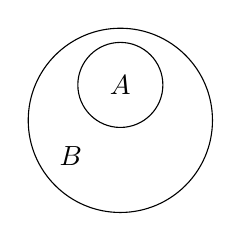
\begin{tikzpicture}[>=latex, scale=.9]
\draw (0,0) circle (.6);
\draw (0,-.5) circle (1.3);
\node at (0,0){$A$};
\node at (-.7,-1){$B$};
    \end{tikzpicture}
    \caption{}
    \end{minipage}
    \begin{minipage}[t]{0.48\textwidth}
    \centering
    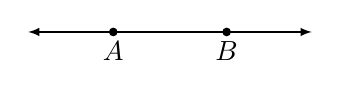
\begin{tikzpicture}[>=latex, scale=.9]
\draw[<->](-2,1)--(2,1);
\draw (-.8,1) [fill=black]circle (1.5pt)node[below]{$A$};
\draw (.8,1) [fill=black]circle (1.5pt)node[below]{$B$};
    \end{tikzpicture}
    \caption{}
    \end{minipage}
    \end{figure}

在图2.4中,$\overline{AB}$上的点都是直线$AB$上的点,但是直线$AB$上的点却还有很多不属于$\overline{AB}$, 所以$\overline{AB}$是直线$AB$的真子集,记作:
\[\overline{AB}\subset \text{直线}AB\]

这里我们要提醒同学们注意区分“属于”关系和“含于”关系。“属于”关系是集合的元素与集合本身的关系,但“含于”关系却是集合与集合之间的关系。

例如集合$A=\{3, 4, 5\},\; B=\{3, 4, 5, 6, 7\}$, 对于元素4来说,它和$A$或$B$的关系是“属于”关系,即$4\in A$, $4\in B$; 对于集合$A$与$B$来说,它们的关系却是“含于”关系,即$A\subset B$。

如果两个集合$A$、$B$是由共同的元素所构成的,我们称它们为相等的集合,记作$A=B$. 例如,$\{x,y,z\}=\{y,x, z\}$, $\{+, -, \x, \div \}=\{ \x, -,+,\div\}$等。

如果两个集合$A$、$B$, $A\subseteq B$且$B\subseteq A$, 这就是说$A$的每个元素都是$B$的元素,而$B$的每个元素也都是$A$的元素,显然这两个集合含有相同的元素,则$A=B$. 例如,$A=\{\text{偶数}\}$,$B=\{2n|n\in\mathbb{Z}\}$, 则$A=B$. 事实上$A$, $B$两个集合
就是同一个集合的两种不同描述法。

如果有三个集合$A$、$B$、$C$, $A\subseteq B$且$B\subseteq C$, 那么显然有$A\subseteq C$. 这就是说集合的含于关系具有传递性。

\subsubsection{集合的运算}

\paragraph{交集}
由集合$A$与集合$B$的公共元素所成的集合叫做集合$A$与集合$B$的交集(或交)。记为:
$A\cap B$,读为$A$交$B$.
\begin{figure}[htp]\centering
    \begin{minipage}[t]{0.48\textwidth}
    \centering
\begin{tikzpicture}[>=latex, scale=1]
    \draw (0,0)node{$A$} circle(.75);
    \draw (1.3,0)node{$B$} circle (1);
    \draw[->](.5,-1.3)node[below]{$A\cap B$}--(.5,-.7);
    \clip {(0,0) circle (.75)};
    \fill[pattern=north east lines] {(1.3,0) circle (1)};
    
    \end{tikzpicture}
    \caption{}
    \end{minipage}
    \begin{minipage}[t]{0.48\textwidth}
    \centering
    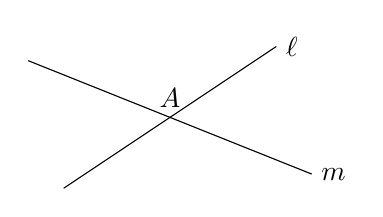
\begin{tikzpicture}[>=latex, scale=.9]
\draw (-2,.8)--(2,-.8)node[right]{$m$};
\draw (-1.5,-1)--(1.5,1)node[right]{$\ell$};
\node at (0,0)[above]{$A$};
    \end{tikzpicture}
    \caption{}
    \end{minipage}
    \end{figure}


两个集合$A$、$B$的交集用维恩图来示意,如图2.5中的阴影部分就表示$A\cap B$.

若$A=\{ a, b, c, d \}$, $B=\{ c, d, e\}$, 则$A\cap B=\{c,d\}$。

在图2.6中,直线$\ell$与直线$m$的交集是$A$点,即$\ell \cap m=\{A\text{点}\}$。
\begin{figure}[htp]\centering
    \begin{minipage}[t]{0.48\textwidth}
    \centering
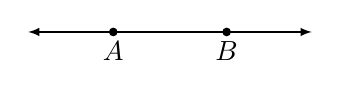
\begin{tikzpicture}[>=latex, scale=.9]
\draw[<->](-2,1)--(2,1);
\draw (-.8,1) [fill=black]circle (1.5pt)node[below]{$A$};
\draw (.8,1) [fill=black]circle (1.5pt)node[below]{$B$};
    \end{tikzpicture}
    \caption{}
    \end{minipage}
    \begin{minipage}[t]{0.48\textwidth}
    \centering
    \begin{tikzpicture}[>=latex, scale=.9]

    \end{tikzpicture}
    \caption{}
    \end{minipage}
    \end{figure}

在图2.7中,$\overline{AB}$是射线$AB$和射线$BA$的交集,即:
\[\overline{AB}=\text{射线}AB\cap \text{射线}BA\]

一条直线把一个平面分成两部分,其中每一部分都叫做半平面,这条直线叫作半平面的界。图2.8中,$\angle AOB$的内部是以直线$OA$为界含有射线$OB$的半平面与以直线$OB$为界含有射线$OA$的半平面的交集(即图中的阴影部分)。

\begin{figure}[htp]\centering
    \begin{minipage}[t]{0.48\textwidth}
    \centering
\begin{tikzpicture}[>=latex, scale=1]
\fill[draw, pattern=north east lines] (0,0)node[fill=white]{$A$} circle(.75);
\fill[draw, pattern=north east lines]  (1.3,0)node[fill=white]{$B$} circle (1);
    \end{tikzpicture}
    \caption{}
    \end{minipage}
    \begin{minipage}[t]{0.48\textwidth}
    \centering
    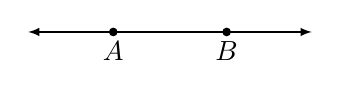
\begin{tikzpicture}[>=latex, scale=.9]
\draw[<->](-2,1)--(2,1);
\draw (-.8,1) [fill=black]circle (1.5pt)node[below]{$A$};
\draw (.8,1) [fill=black]circle (1.5pt)node[below]{$B$};
    \end{tikzpicture}
    \caption{}
    \end{minipage}
    \end{figure}

显然,若$A\subseteq B$, 则$A\cap B=A$, 反之,若$A\cap B=A$, 则$A\subseteq B$.

\paragraph{并集}
由集合$A$的元素或集合$B$的元素合并而成的
集合叫做集合$A$与集合$B$的并集(或并)记为:
$A\cup B$,读为A并B。

集合$A$与集合$B$的并集用维恩图示意,如图2.9所示,图中的阴影部分就表示$A\cup B$.

如果$A=\{1, 2, 3\}$, $B=\{3, 4, 5\}$, 那么$A\cup B= \{1, 2, 3, 4, 5\}$.

\begin{rmk}
    在求上述$A$、$B$的并集时,虽然$A$与$B$含有共同的元素3, 但在$A\cup B$中3只取一次。
\end{rmk}

如果$A_+=\{x|x\text{是实数,且}x\ge 5\}$,$A_-=\{x|x\text{是实数,且}x\le -5\}$,$A=\{x|x^2\ge 25\}$,那么$A_+\cup A_-=A$。

在图2.10中,直线$AB$是射线$AB$和射线$BA$的并集,即
\[\text{直线}AB=\text{射线}AB \cup \text{射线}BA\]

\paragraph{空集}
为了使集合$A$和集合$B$的交集$A\cap B$在集合$A$与集合$B$不含有任何公共元素时仍有意义,我们自然想到:这时的$A\cap B$应是一个不含有任何元素的集合。因此,我们把这种不含任何元素的集合叫做\textbf{空集},并用符号$\emptyset$表示。

由空集的意义可知,对任何一个集合$P$, 都有$P\cap \emptyset=\emptyset$, $P\cup\emptyset=P$成立,并且空集是任何一个集合$P$的子集。即:$P\supseteq \emptyset$

如果$A=\{\text{奇数}\}$,$B=\{\text{偶数}\}$,那么$A\cap B=\emptyset$。

在图2.11中,若$\odot O_1$和$\odot O_2$相离,则$\odot O_1\cap \odot O_2=\emptyset$
\begin{figure}[htp]
    \centering
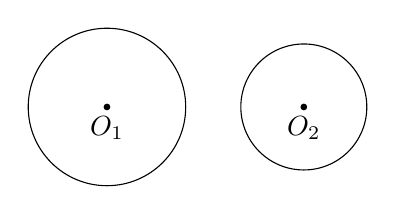
\begin{tikzpicture}
\draw (0,0)node[below]{$O_1$} circle (1);
\draw (2.5,0)node[below]{$O_2$} circle (.8);
\draw (0,0) [fill=black] circle(1pt); 
\draw (2.5,0) [fill=black] circle(1pt); 
\end{tikzpicture}
    \caption{}
\end{figure}

如果直线$a\parallel$直线$b$, 那么$a\cap b=\emptyset$.

\paragraph{基集与补集}

如果我们所讨论的集合都是一个给定集合的子集,我们就称这个给定集合为\textbf{基集},通常用符号$I$表示基集。

例如,我们所讨论的集合是$\emptyset$、$\{1\}$、$\{2\}$、$\{3\}$、$\{1, 2\}$、$\{2, 3\}$、$\{1, 3\}$和$\{1, 2, 3\}$时,因为上述集合都是集合$\{1, 2, 3\}$的子集,所以我们称$\{1, 2, 3\}$为基集。

又因为平面和平面上的几何图形都是点的集合,那么平面几何所讨论的图形都可以看作是某平面上所有点的集合的
子集,这时,我们把平面叫做基集。

在代数中,当我们讨论有理数运算时,全体有理数就是基集。

如果$A\subseteq I$, 在基集$I$中所有不属于$A$的元素所构成的集
合叫做$A$的\text{补集},以符号“$A^c$”表示,读为$A$补。因此,




\begin{figure}[htp]\centering
    \begin{minipage}[t]{0.48\textwidth}
    \centering
\begin{tikzpicture}[>=latex, scale=1.3]
\fill[pattern=north east lines, draw](0,0) rectangle (3.5,2.5);
\draw [fill=white](1.5,1)node{$A$} circle (.6);
\node at (3,2)[fill=white]{$I$};
\node at (3,1)[fill=white]{$A^c$};
    \end{tikzpicture}
    \caption{}
    \end{minipage}
    \begin{minipage}[t]{0.48\textwidth}
    \centering
    \begin{tikzpicture}[>=latex, scale=1.3]
\fill[pattern=north east lines, draw](0,0) rectangle (3.5,2.5);
\draw [fill=white](1.5,1)node[left]{$O$} circle (.6);
\node at (1.5,.75){$B^c=A$};
\draw [->](1.5,1)--node[above]{3}+(30:.6);
\node at (1.2,1.35){$A$};
\node at (3,2)[fill=white]{$P$};
\node at (2.8,1)[fill=white]{$A^c=B$};
\node at (.5,.5)[fill=white]{$B$};
    \end{tikzpicture}
    \caption{}
    \end{minipage}
    \end{figure}



\begin{figure}[htp]\centering
    \begin{minipage}[t]{0.48\textwidth}
    \centering
\begin{tikzpicture}[>=latex, scale=1.3]
\fill[pattern=north east lines, draw](0,0) rectangle (3.5,2.5);
\draw [fill=white](1.8,1.2)node{$A$} circle (1);
\draw [fill=white](2,1)node{$A$} circle (.5);
\node at (1.2,1.4){$B$};
\node at (3.1,.25)[fill=white]{$B^c$};
\node at (.5,2.2)[fill=white]{$I$};

    \end{tikzpicture}
    \caption{}
    \end{minipage}
    \begin{minipage}[t]{0.48\textwidth}
    \centering
    \begin{tikzpicture}[>=latex, scale=1.3]
\fill[pattern=north east lines, draw](0,0) rectangle (3.5,2.5);
\draw [fill=white](1.8,1.2) circle (1);
\draw [fill=white](2,1)node{$A$} circle (.5);
\node at (3.1,.25)[fill=white]{$B^c$};
\node at (.5,2.2)[fill=white]{$I$};
\node at (1.2,1.4){$A^c$};

    \end{tikzpicture}
    \caption{}
    \end{minipage}
    \end{figure}

























